\chapter{Algoritmi su stringhe}\label{algoritmi-su-stringhe}

\section{Il problema del matching esatto}\label{il-problema-del-matching-esatto}

Si ha un pattern \emph{P} di lunghezza \emph{m} e un testo \emph{T} in
cui cercare il pattern di lunghezza $n \geq m$.

Un esempio di problema è la ricerca del pattern \emph{P = aba} in
\emph{T=bbabaxababay}. In questo caso ci sono 3 occorrenze del pattern,
che si sovrappongono tra loro.

Risolvere questo problema in modo efficiente è di importanza chiave dal
momento che tutti i motori di ricerca si basano sul pattern matching
esatto o approssimato. Un altro campo in cui è utile il pattern matching
è nella bioinformatica, infatti, il DNA umano può essere visto come una
stringa di 4 miliardi di caratteri.

\subsection{Notazione utilizzata}\label{notazione-utilizzata}

Una stringa è composta da un insieme \emph{Sigma} di simboli
distinguibili e che prendono il nome di \textbf{caratteri dell'alfabeto}.

L'alfabeto, ovvero l'insieme di simboli, può essere finito oppure
infinito ed è dotato di un ordine totale tra i vari simboli.

Una successione finita dei caratteri dell'alfabeto prende il nome di
\textbf{stringa} e i caratteri che la compongono vengono indicizzati a
partire da 1.

$$
X = x_1 \ldots x_n
$$

$|X|$ indica la lunghezza di una stringa e nel
caso questa sia 0, la stringa è vuota e viene rappresentata con
$\epsilon$.

Due stringhe possono essere concatenate tra loro:

$$
X \cdot Y = x_1\ldots x_ny_1\ldots y_m
$$

e $\epsilon$ è l'elemento neutro per la concatenazione, dal momento
che la concatenazione della stringa vuota ad un'altra stringa è uguale
alla stringa di partenza.

La concatenazione multipla della stessa stringa viene indicata con
l'esponenziale:

$$
X^k = \underbrace{X \cdot \ldots \cdot X}_{k}
$$

Una \textbf{sottostringa} di una stringa \emph{X} è una stringa
\emph{Y}, tale che
$X = Z \cdot Y \cdot W$ per
qualche \emph{Z, W}.

Ogni terna \emph{(Z,Y,W)} prende il nome di \textbf{occorrenza} di
\emph{Y} in \emph{X} e si dice che la stringa \emph{Y} \textbf{occorre}
in \emph{X} nella posizione $i = |Z| + 1$.
In particolare si ha:

$$
X = Z \cdot Y \cdot W = X[1,i-1]X[i,j]X[j+1,n]
$$

Se la stringa $Z = \epsilon$, \emph{Y} prende il nome di
\textbf{prefisso}, mentre se $W=\epsilon$, \emph{Y} prende il nome
di \textbf{suffisso}.

Se la stringa \emph{Y} è sia prefisso che suffisso di \emph{X}, allora
\emph{Y} è un \textbf{bordo} della stringa \emph{X} e si ha che

$$
Y = X[1,m] = X[n-m+1,n]
$$

Prefissi, suffissi, bordi e sottostringhe vengono detti \textbf{propri}
se sono $\neq \epsilon$ e $\neq X$, altrimenti vengono detti
\textbf{degeneri}.

\subsubsection{Periodo}\label{periodo}

Se \emph{Y} è un bordo di \emph{X} allora esistono \emph{Z} e \emph{W}
tali che $X = Z \cdot Y = Y \cdot W$ con
$|Z| =|W| = p = n - m$.
\emph{p} prende il nome di \textbf{periodo} della stringa \emph{X}.

Un periodo si dice \textbf{proprio} se $0 < p <n$.

\paragraph{Lemma - Periodi e Bordi}\label{lemma---origine-del-periodo}

Il nome periodo deriva dal fatto che se $X = x_1x_2\ldots x_n$ ha
come bordo \emph{Y} di lunghezza \emph{m}. Allora $x_i = x_{i+p}$ per
ogni \emph{i} tale che $1 \leq i \leq n-p$. 
Viceversa se $x_i = x_{i+p}$, per ogni \emph{i} tale che $1 \leq i \leq n - p$ allora
$Y = X[1,n-p]$ è un bordo di \emph{X}.

\subparagraph{Dimostrazione}\label{dimostrazione}

Per definizione di bordo, \emph{Y} è un bordo di \emph{Z} se e solo se

$$
Y = X[1,m]=X[n-m+1,n]
$$

Ma $X[1,m] = X[n-m+1,n]$ se e solo se sono uguali i corrispondenti caratteri $x_i$ e $x_{i+n-m}$ per $i = 1, \ldots, m$, ma questo è come dire $x_i = x_{i+p} \forall i \: = 1,\ldots, n-p $ con $p  = n-m$. 

Pertanto, segue che la stringa \textit{X} di lunghezza \textit{n} ha un bordo \textit{Y} se e solo se \textit{p = n-m} è un periodo delle stringa.

Una stringa \emph{X} viene detta \textbf{periodica} se
$0 \leq 2p \leq n$ ovvero se c'è un bordo di lunghezza
$m  < n \leq 2m$.

\paragraph{Lemma - Concatenazione di stringhe periodiche}\label{lemma---concatenazione-di-stringhe-periodiche}

Siano \emph{X} e \emph{Y} due stringhe con periodo \emph{p} tali che $X = \alpha\gamma$ e $Y = \gamma\beta$ con $|\gamma| \geq p$.

La stringa $Z = \alpha\gamma\beta$ ha anch'essa periodo \emph{p}.

\begin{figure}[htbp]
\centering
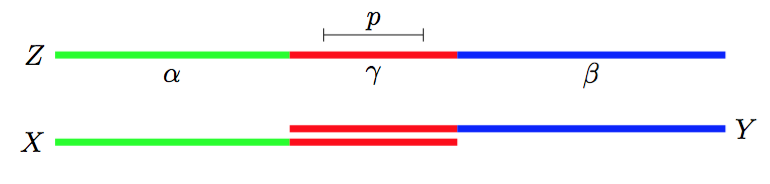
\includegraphics[width=.7\textwidth]{./notes/immagini/l10-fig1.png}
\end{figure}

\subparagraph{Dimostrazione}\label{dimostrazione-1}

Siano $ z_i $ e $ z_{i+p} $ dure caratteri di \textit{Z} a distanza \textit{p}. Siccome $ |\gamma|  \geq p$, i due caratteri possono essere appartenenti solamente o a \textit{X} o a \textit{Y} e mai ad entrambe le stringhe contemporaneamente. 
Pertanto dal momento che sia \textit{X} sia \textit{Y} hanno periodo \textit{p}, i due caratteri devono essere per forza uguali.

Da questo segue il lemma di periodicità che afferma che due periodi distinti \emph{p} e \emph{q} non possono coesistere troppo a lungo in
una stessa stringa senza che la stringa abbia anche periodo \emph{MCD(p,q)}.

\paragraph{Lemma - Lemma di periodicità}\label{lemma---lemma-di-periodicituxe0}

Sia \emph{X} una stringa di lunghezza \emph{n} con due periodi \emph{p}
e \emph{q} non entrambi nulli.

Se $n \geq p + q - MCD(p,q)$ allora la stringa \emph{X} ha anche periodo \emph{MCD(p,q)}.

\begin{figure}[htbp]
\centering
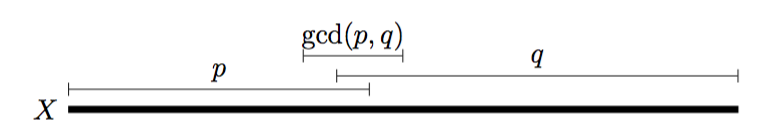
\includegraphics[width=.7\textwidth]{./notes/immagini/l10-fig2.png}
\caption{}
\end{figure}

\subparagraph{Dimostrazione}\label{dimostrazione-2}

Supponendo che $p \leq q$, la dimostrazione viene fatta per induzione su \emph{p+q}.

$(p+q = 1)$ 

Se \emph{p=0} oppure \emph{p=q=0} allora \emph{MCD(p,q) = q} e dunque
\emph{X} ha periodo \emph{MCD(p,q)} perché ha periodo \emph{q}.

$(p+q > 1)$

Se \emph{p=0} o \emph{p=q} vale ancora il caso base.

Se $1 \leq p < q$, si ha che la stringa \emph{X} ha bordi $\alpha$ e $\beta$ di lunghezza \emph{n-p} e \emph{n-q}, questo per il primo lemma dimostrato.

\begin{figure}[htbp]
\centering
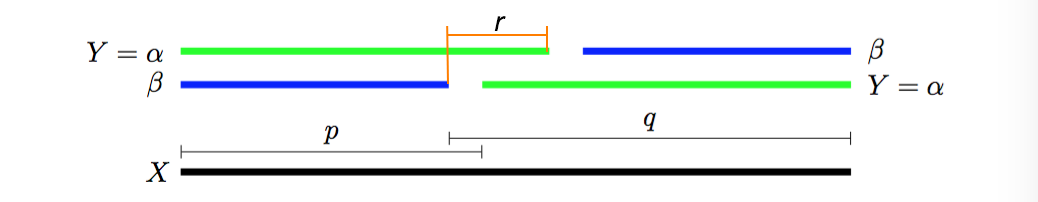
\includegraphics[width=.7\textwidth]{./notes/immagini/l10-fig3.png}
\caption{In verde la stringa $\alpha$ che si ripete con periodo
\emph{p}. In blu la stringa $\beta$ che si ripete con periodo
\emph{q}}
\end{figure}

La stringa $\beta$ essendo bordo di \emph{X} è anche bordo $\alpha$ dal momento che $\alpha$ è un bordo di \emph{X}, pertanto $\alpha$ ha periodo $r = |\alpha| - |\beta| = q -p$.

Si ha che $p+r < p + q$ e \emph{MCD(p,r) = MCD(p,q)}, quindi per ipotesi induttiva

$$
|\alpha| = n - p \geq q - MCD(p,q) = p+r+MCD(p,q)
$$

$ \alpha $ ha quindi come periodo sia \textit{r} (a causa di $ \beta $), sia \textit{p} (per ipotesi), ovvero ha periodo \textit{MCD(p,r)} che per come è definito \textit{r} è uguale a \textit{MCD(p,r)}.

Si ha quindi che

\begin{align*}
	2|\alpha| &= (n-p) + (n-p) \\
					 &\geq q - MCD(p,q) + (n-p) \\
					 &\geq n
\end{align*}

perché $ p < q $ per ipotesi e $ MCD(p,q) \leq q - p $ per le proprietà del massimo comun divisore.

Questo implica che il prefisso $ \alpha $ di \textit{X} e il suffisso $ \alpha $ di \textit{X} coprono tutto \textit{X} e pertanto le due stringhe devono sovrapporsi\footnote{Non è possibile applicare il lemma della concatenazione perché non si sa di quanto queste stringhe si sovrappongono.} oppure $ X = \alpha\alpha $.

Presi quindi due caratteri $ x_i $ e $ x_j $ della stringa \textit{X}, tali che $ j - i = MCD(p,q) $ può succedere che i due caratteri appartengano alla stessa $ \alpha $ e quindi siano uguali, perché $ \alpha $ ha periodo $ r = MCD(p,q) $ oppure che $x_i \in \alpha_{(prefisso)} \text{ e } x_j \in \alpha_{(suffisso)} $.

\begin{figure}[htbp]
	\centering
	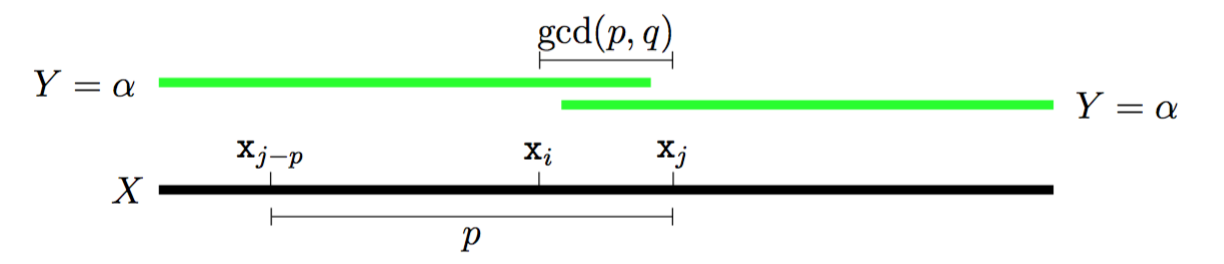
\includegraphics[width=.7\textwidth]{./notes/immagini/l10-fig4.png}
\end{figure}


In questo caso si ha che $ j > n - |\alpha| = p $ e quindi $ j - p \geq 1$. Si può quindi considerare il carattere $ x_{j-p} = x_j$ per via del periodo \textit{p} di $ \alpha $ e che risulta appartenere a $ \alpha_{(prefisso)} $ perché $ p \geq MCD(p,q) $.

La distanza tra $ x_{j-p} \text{ e } x_i$ è \textit{p - MCD(p,q)}, che per definizione è un multiplo di \textit{MCD(p,q)}, pertanto si ha che $ x_{j-p} \text{ e } x_i$ appartengono ad $ \alpha_{(prefisso)} $ che ha periodo \textit{MCD(p,q)}, pertanto $ x_{j-p} = x_i = x_j $ e di conseguenza \textit{X} ha periodo \textit{MCD(p,q)}.

